\section{Распознавание речи и голосовое управление (вариант 8)}
\label{sec:recognize}

\subsection{Постановка задачи}

В соответствии с вариантами~8 и~7 система расширена подсистемой
автоматизированного распознавания речи (speech-to-text, STT): пользователь
произносит голосовую команду на \textbf{английском} или \textbf{французском}
языке, система распознавает речь, сопоставляет её с \textbf{списком
операций}, выполняет соответствующую реакцию и \textbf{уведомляет}
пользователя о происходящем. Тематика "--- литературные эссе; синтез и
распознавание выполняются \textbf{полностью офлайн} (без облачных API).

Минимальные требования методических указаний закрыты так:

\begin{itemize}
	\item \textbf{Список операций} "--- 16 фиксированных операций
	      (поиск, реферирование, перевод, озвучивание, определение языка,
	      список команд, навигация на все 10 страниц интерфейса,
	      справка); \textbf{триггерные
	      фразы EN/FR редактируются пользователем}, поведение операции
	      при этом не меняется;
	\item \textbf{Автоматическая реакция} "--- после сопоставления вызывается
	      целевой сервис (поиск / реферирование / перевод / детектор языка)
	      или клиентская навигация; пользователь получает двуязычное
	      уведомление (toast + опционально голосом через подсистему синтеза
	      речи);
	\item \textbf{Настройка ЕЯ} "--- селектор EN/FR выбирает модель Vosk
	      и набор фраз для сопоставления.
\end{itemize}

Движок "--- \textbf{Vosk} (Kaldi, офлайн): модели
\texttt{vosk-model-small-en-us-0.15} и \texttt{vosk-model-small-fr-0.22}
($\approx$40~МБ, скачиваются при сборке образа).

\subsection{Структура системы, технологии и методики}

Подсистема реализована шестью модулями (каталог \texttt{backend/}):

\begin{itemize}
	\item \texttt{stt/engines.py} "--- загрузка и кэш моделей Vosk
	      (блокировка потоков), декодирование WAV $\to$ mono int16
	      16~кГц (линейная интерполяция), \textbf{двухпроходное}
	      распознавание: free (открытый словарь, для аргументов) и
	      constrained (ограничение словаря словами всех фраз "--- для
	      матчинга), лимит 30~с;
	\item \texttt{stt/commands.py} "--- реестр фиксированных операций и
	      редактируемых фраз; хранение в
	      \texttt{backend/data/stt\_commands.json} (кэш по mtime,
	      атомарная запись, seed-значения при отсутствии файла,
	      merge новых \texttt{open\_*}-операций в старый JSON);
	\item \texttt{stt/matcher.py} "--- нормализация (нижний регистр,
	      снятие акцентов NFD "--- важно: Vosk часто отбрасывает
	      акценты French, пунктуация) и сопоставление с фразами;
	\item \texttt{services/stt\_service.py} "--- валидация, двухпроходный
	      вызов движка, выбор лучшего совпадения, диспетчер операций,
	      библиотека уведомлений EN/FR, метрики;
	\item \texttt{controllers/stt.py} "--- четыре REST-эндпоинта
	      с Blueprint-обработчиками ошибок;
	\item \texttt{frontend/stt.html} + \texttt{frontend/js/stt.js} "--- UI:
	      запись с микрофона, селектор ЕЯ, выбор документа для
	      реферирования, лог, карточки статистики, toast, редактор фраз,
	      голосовое уведомление через существующий TTS.
\end{itemize}

Архитектура показана на рисунке~\ref{fig:stt_arch}
(исходник "--- \texttt{plantuml/architecture\_stt.puml}).

\begin{figure}[H]
	\centering
	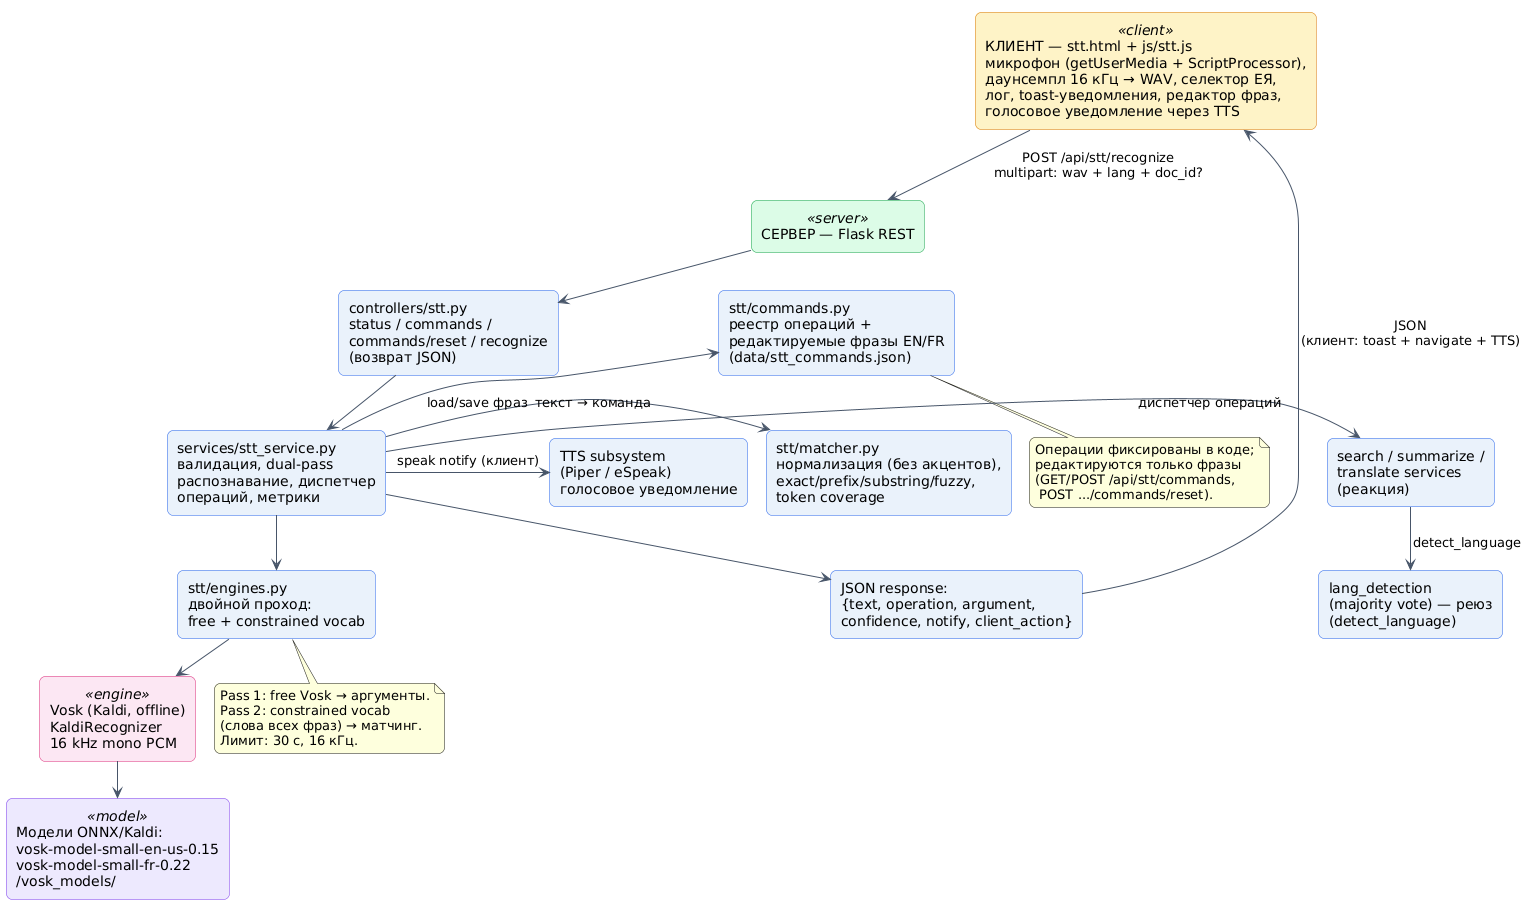
\includegraphics[width=1.0\textwidth]{png/architecture_stt.png}
	\caption{Архитектура подсистемы распознавания речи.}
	\label{fig:stt_arch}
\end{figure}

Захват речи выполняется в браузере: \texttt{getUserMedia} $\to$
\texttt{ScriptProcessor} (Float32-чанки) $\to$ даунсемпл до 16~кГц mono
$\to$ WAV $\to$ \texttt{POST /api/stt/recognize} (multipart). Сервер
не зависит от ffmpeg/webm: на входе "--- WAV PCM16.

\subsection{Основные алгоритмы}

Блок-схема алгоритма голосовой команды приведена на
рисунке~\ref{fig:stt_activity}
(исходник "--- \texttt{plantuml/activity\_stt.puml}).

\begin{figure}[H]
	\centering
	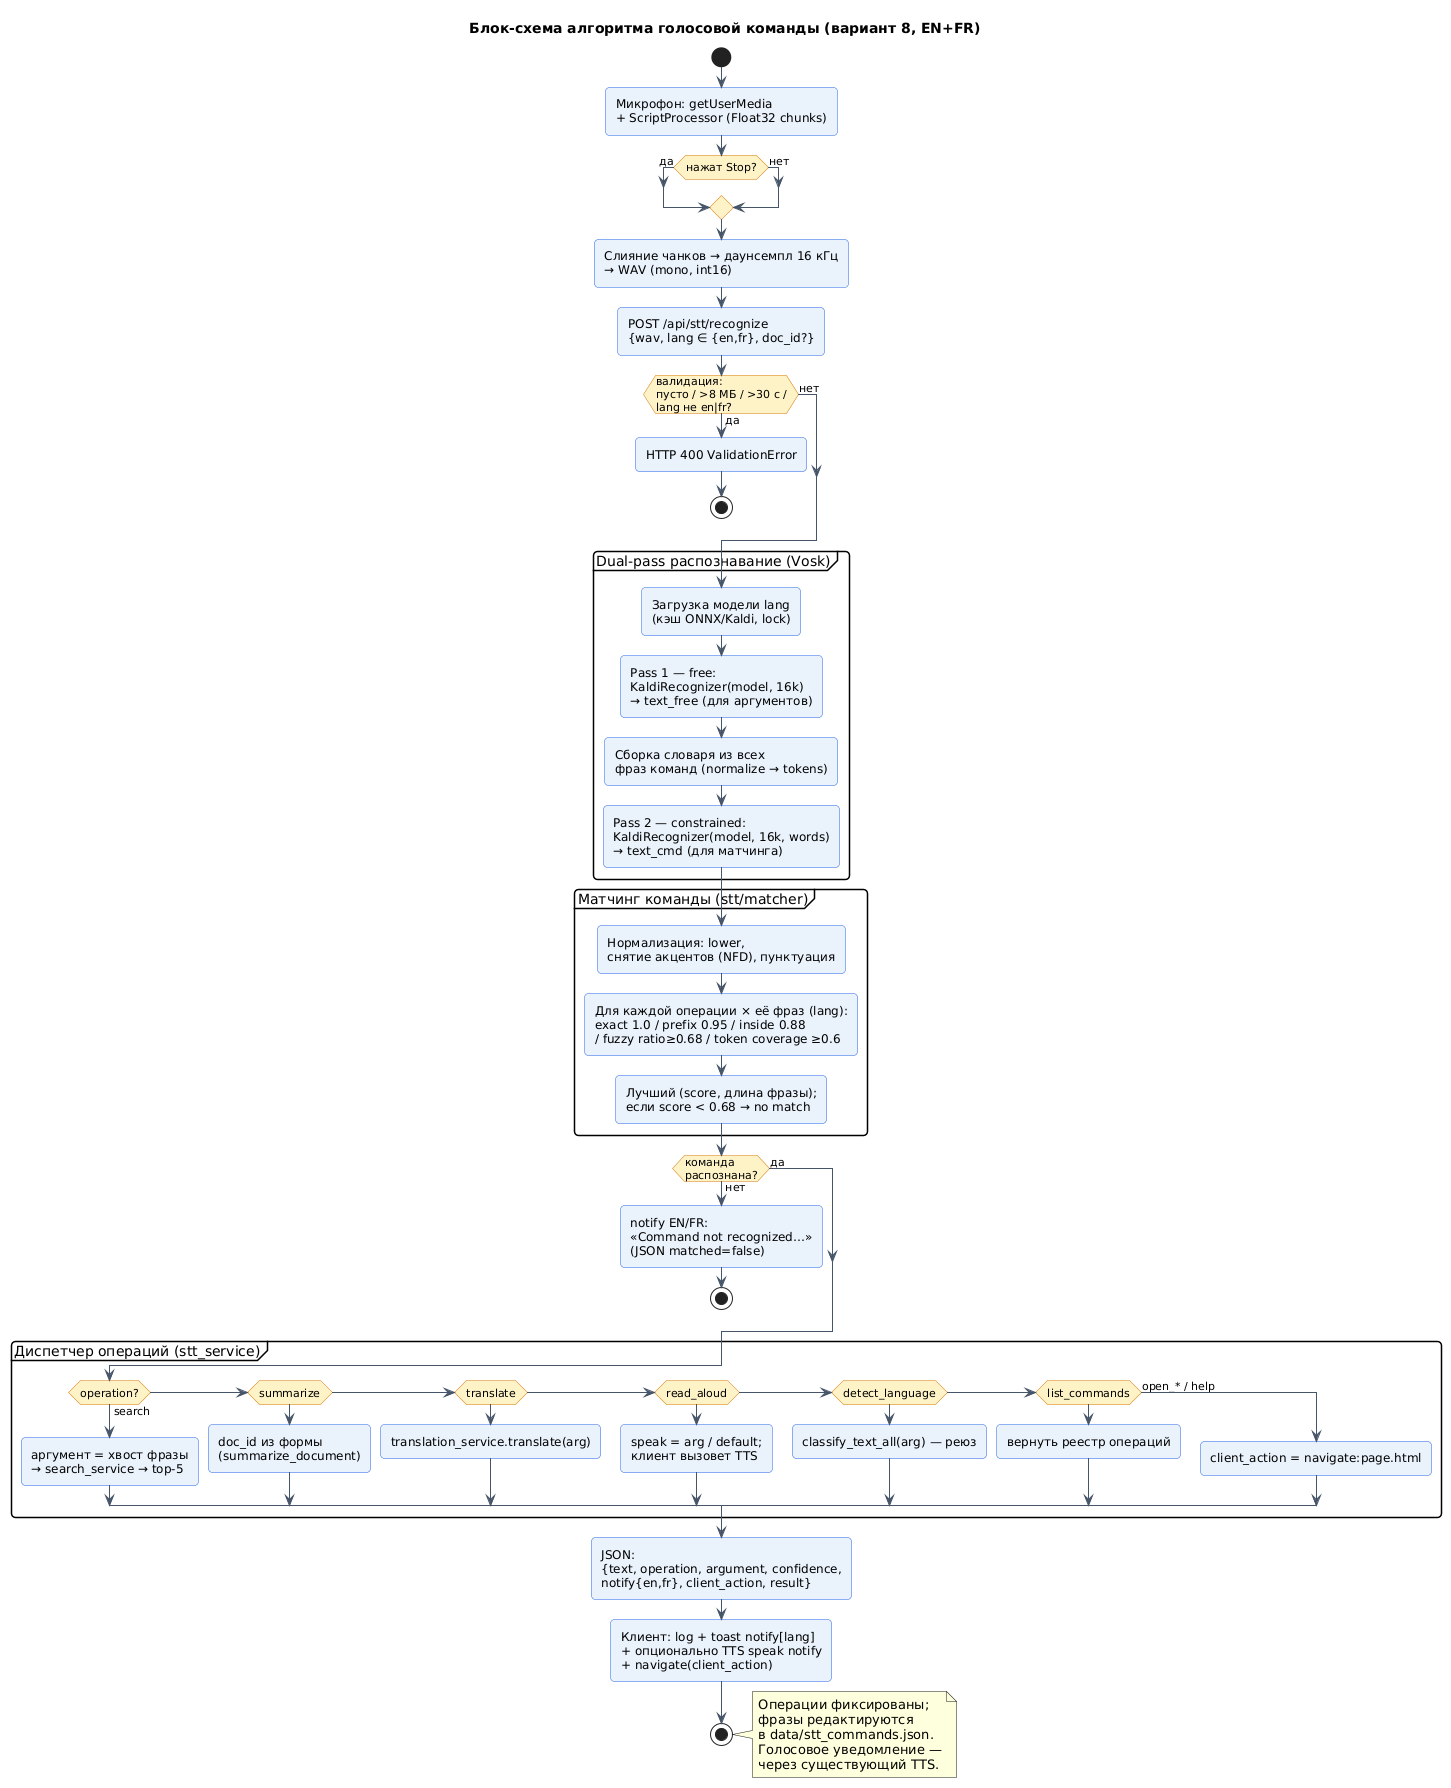
\includegraphics[width=0.72\textwidth]{png/activity_stt.png}
	\caption{Блок-схема алгоритма голосовой команды.}
	\label{fig:stt_activity}
\end{figure}

\subsubsection{Двухпроходное распознавание}

Один и тот же PCM-буфер обрабатывается дважды:

\begin{enumerate}
	\item \textbf{Pass 1 (free)} --- \texttt{KaldiRecognizer(model, 16000)}
	      без ограничений: открытый словарь для извлечения аргументов
	      («search for \emph{hamlet}», «traduire \emph{bonjour}»);
	\item \textbf{Pass 2 (constrained)} ---
	      \texttt{KaldiRecognizer(model, 16000, words)}, где \texttt{words}
	      "--- JSON-список всех токенов фраз выбранного языка
	      (\texttt{commands.vocab\_words}). Ограничение словаря резко
	      повышает точность на коротких командах («help»/«aide»),
	      которые free-проход часто искажает.
\end{enumerate}

Матчинг выполняется по обоим транскриптам; берётся совпадение с большим
\texttt{confidence}, аргумент предпочитается из free-транскрипта.
Такая методика даёт accuracy 25/25 на эталонных фразах (см. тесты).

\subsubsection{Сопоставление с редактируемыми фразами}

Для каждой операции $\times$ её фразы на выбранном ЕЯ вычисляется score
(таблица~\ref{tab:stt_scores}); лучшая пара "--- по
\texttt{(score, длина\_фразы)}, порог совпадения 0,68.

\begin{table}[H]
	\caption{Правила оценки совпадения фразы и транскрипта.}
	\label{tab:stt_scores}
	\begin{tabular}{|p{0.32\textwidth}|p{0.12\textwidth}|p{0.44\textwidth}|}
		\hline
		Условие & Score & Комментарий \\ \hline
		транскрипт == фраза & 1,00 & точное совпадение \\
		префикс \texttt{text startswith phrase} & 0,95 & аргумент "--- хвост \\
		фраза внутри текста & 0,88 & слово-в-слово \\
		\texttt{SequenceMatcher} ratio $\ge$ 0,68 & $0{,}92 \times$ ratio & нечёткое \\
		token coverage $\ge$ 0,6 ( $\ge$ 2 токенов) & $0{,}70+0{,}25 \times$ cov & ASR сохранил содержательные слова \\
		score $<$ 0,68 & --- & no match \\ \hline
	\end{tabular}
\end{table}

Длинные фразы проверяются раньше коротких, поэтому «search for»
выигрывает у «search». Для команд с аргументом
(\texttt{takes\_argument=true}) хвост после фразы становится параметром
(«search for hamlet» $\to$ query=\texttt{hamlet}).

\subsubsection{Диспетчер операций и уведомление}

Сценарий вызова "--- диаграмма последовательности на
рисунке~\ref{fig:stt_seq}
(исходник "--- \texttt{plantuml/sequence\_stt.puml}).

\begin{figure}[H]
	\centering
	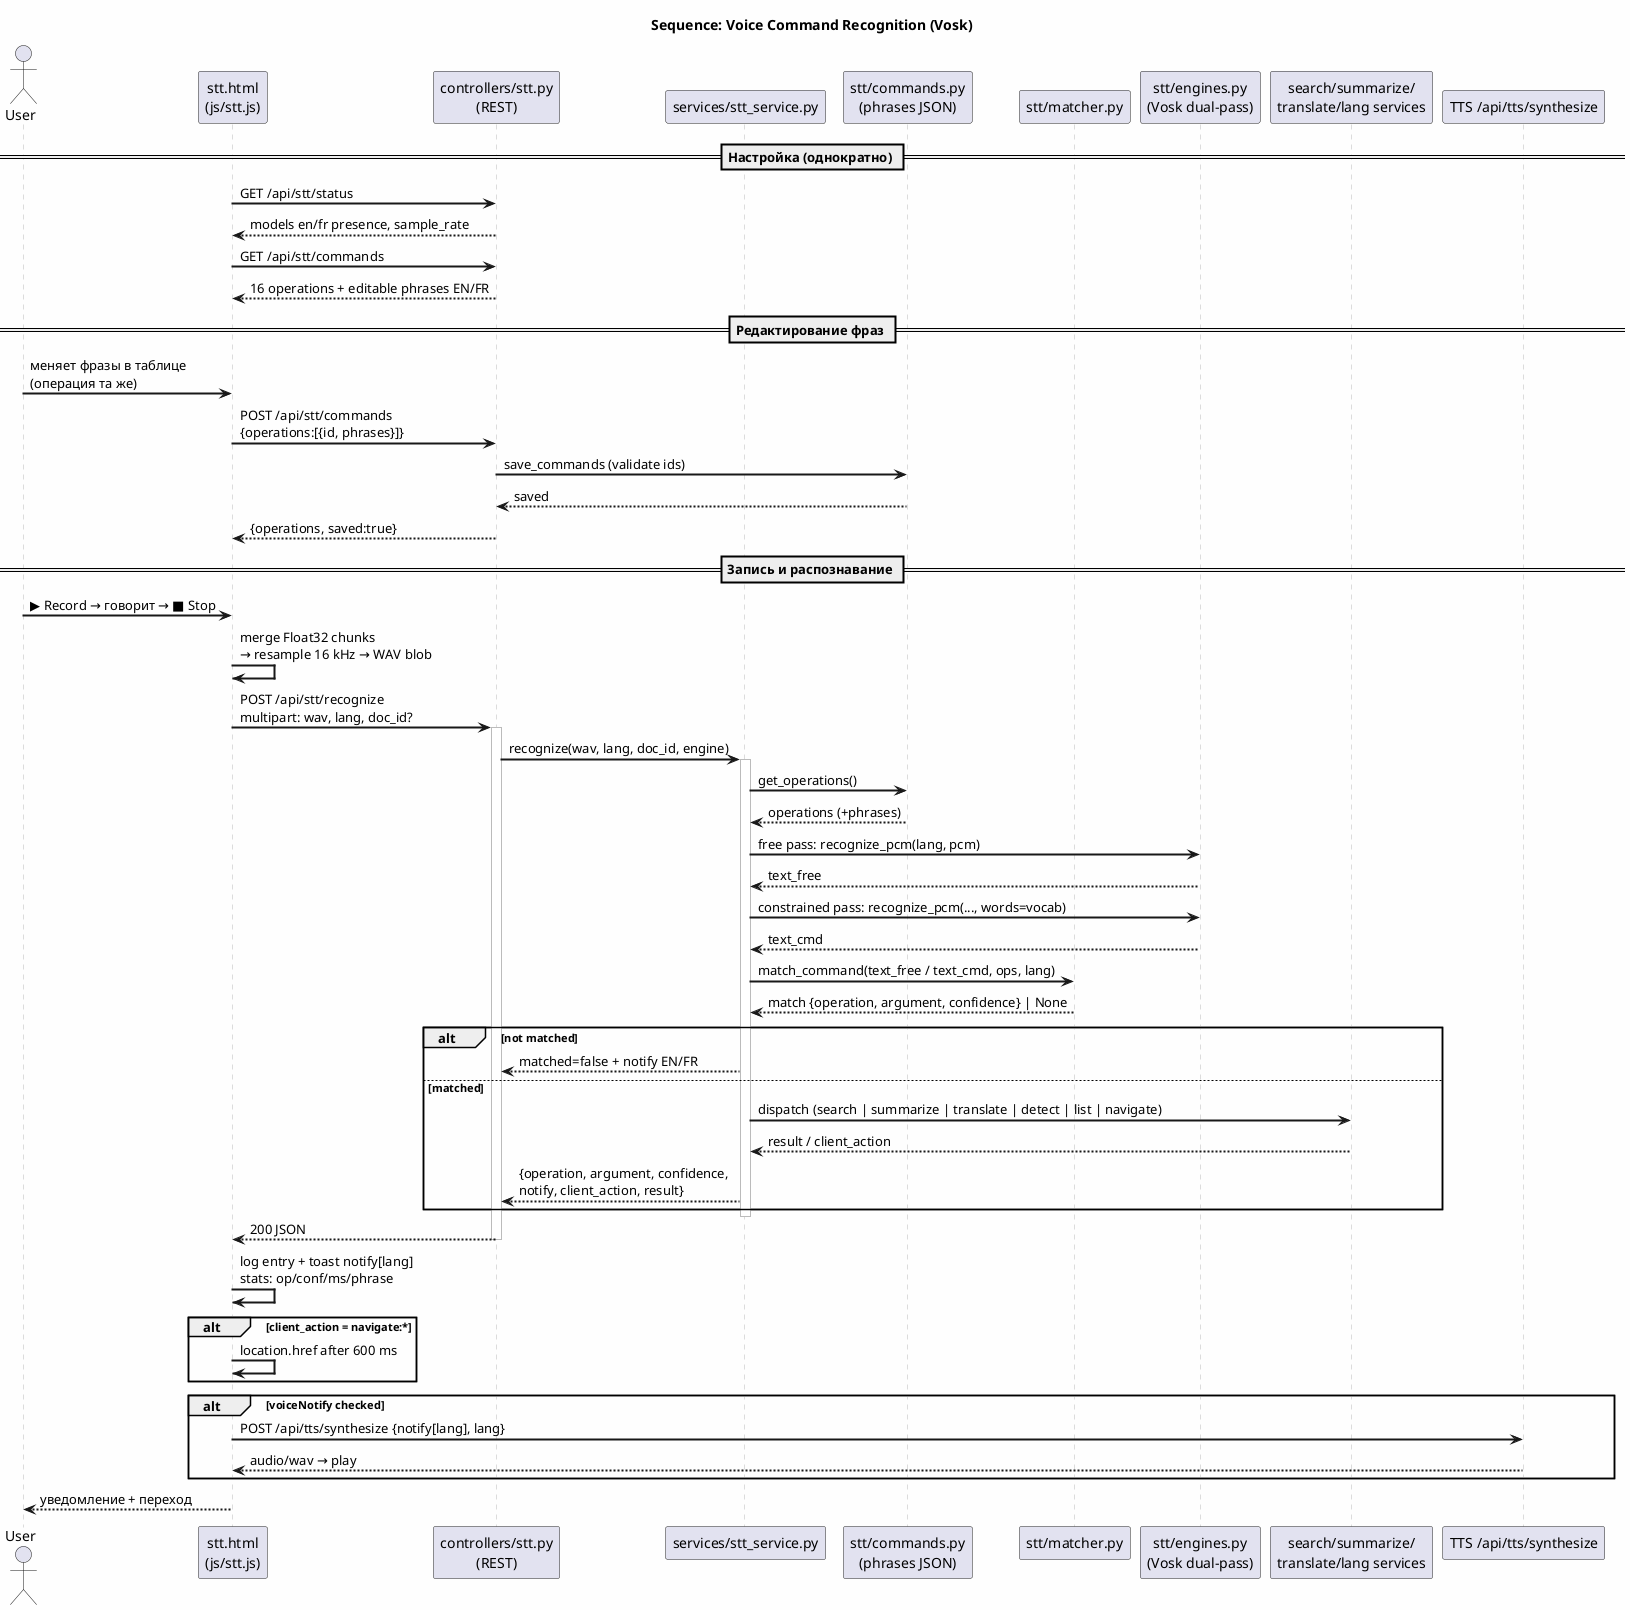
\includegraphics[width=1.0\textwidth]{png/sequence_stt.png}
	\caption{Диаграмма последовательности: голосовая команда.}
	\label{fig:stt_seq}
\end{figure}

Реакции операций (фиксированы в коде, фразы --- нет):

\begin{table}[H]
	\caption{Операции голосового управления и их реакции.}
	\label{tab:stt_ops}
	\begin{tabular}{|p{0.22\textwidth}|p{0.40\textwidth}|p{0.28\textwidth}|}
		\hline
		Операция & Реакция & Аргумент \\ \hline
		\texttt{search} & \texttt{search\_service}, top-5, навигация на выдачу & хвост фразы \\
		\texttt{summarize} & \texttt{summarize\_document(doc\_id)} из формы & \texttt{doc\_id} \\
		\texttt{translate} & \texttt{translation\_service.translate} & хвост фразы \\
		\texttt{read\_aloud} & текст $\to$ TTS-синтез на клиенте & хвост / default \\
		\texttt{detect\_language} & \texttt{classify\_text\_all} (реюз варианта~7) & хвост фразы \\
		\texttt{list\_commands} & вернуть реестр операций, открыть редактор & --- \\
		\texttt{open\_search}, \texttt{open\_documents}, \texttt{open\_summarize},
		\texttt{open\_translate}, \texttt{open\_classify}, \texttt{open\_upload},
		\texttt{open\_metrics}, \texttt{open\_tts}, \texttt{open\_stt},
		\texttt{help} & \texttt{client\_action = navigate:*.html}
		(все 10 страниц) & --- \\ \hline
	\end{tabular}
\end{table}

Ответ сервера: \texttt{\{text, operation, argument, confidence,
matched\_phrase, notify\{en,fr\}, client\_action, result, recognized\_ms\}}.
Клиент пишет лог, показывает toast \texttt{notify[lang]}, опционально
озвучивает его через \texttt{POST /api/tts/synthesize} и выполняет
навигацию. Если аргумент не передан, операция не падает "--- возвращается
подсказка EN/FR («Добавьте запрос после команды…»).

\subsubsection{Редактирование фраз}

\texttt{GET/POST /api/stt/commands}, \texttt{POST /api/stt/commands/reset}.
При сохранении валидируются: известный id операции (набор операций
нельзя расширить/удалить), непустые списки фраз EN и FR, длина фразы
$\le$ 80 символов, отсутствие дубликатов. \texttt{reset} восстанавливает
seed-значения. Файловый доступ защищён \texttt{RLock} (seed при
первом обращении).

\subsection{API методы}

\begin{lstlisting}[caption={HTTP эндпоинты подсистемы распознавания речи.},label={lst:stt_api}]
GET  /api/stt/status           --- наличие моделей Vosk EN/FR, 16 kHz, лимит 30 s
GET  /api/stt/commands         --- операции + редактируемые фразы EN/FR
POST /api/stt/commands         --- сохранить фразы {operations:[{id,phrases}]}
POST /api/stt/commands/reset   --- восстановить фразы по умолчанию
POST /api/stt/recognize        --- multipart: wav, lang=en|fr, doc_id?
                                   => JSON {operation, argument, confidence,
                                     notify, client_action, ...}
\end{lstlisting}

\subsection{Результаты тестирования}

Автотесты (\texttt{/tmp/stt\_test.py} $\to$ \texttt{/tmp/stt\_bench.json}):
эталонные WAV генерируются \textbf{нейро-голосом Piper} через
\texttt{/api/tts/synthesize} (близко к живой речи; формантный eSpeak даёт
$\approx$15\,\% распознавания "--- зафиксировано при отладке),
затем отправляются в \texttt{/api/stt/recognize}.

\textbf{Матчинг команд} "--- таблица~\ref{tab:stt_acc}: \textbf{25/25 (100\,\%)},
15 EN + 10 FR, включая точные фразы, перефразировки («what can you do»,
«faire un résumé») и команды с аргументами.

\begin{table}[H]
	\caption{Ключевые случаи распознавания и сопоставления (фрагмент).}
	\label{tab:stt_acc}
	\begin{tabular}{|l|l|l|l|l|}
		\hline
		ЕЯ & Фраза (факстура Piper) & Операция & Аргумент & Conf \\ \hline
		EN & search for hamlet & search & hamlet & 0,95 \\
		EN & summarize & summarize & --- & 1,00 \\
		EN & detect language this sentence is english & detect\_language & \ldots english & 0,95 \\
		EN & help & help & --- & 1,00 \\
		EN & what can you do & list\_commands & --- & 1,00 \\
		FR & rechercher le bonheur & search & le bonheur & 0,95 \\
		FR & résumer & summarize & --- & 1,00 \\
		FR & lire à voix haute bonjour & read\_aloud & bonjour & 0,95 \\
		FR & quelle est cette langue & detect\_language & --- & 1,00 \\ \hline
	\end{tabular}
\end{table}

\textbf{Задержка распознавания} (тёплая модель, dual-pass, без учёта
записи): EN avg 1086~мс (min 639, max 1523), FR avg 1553~мс
(min 985, max 2476); общий avg 1273~мс; \textbf{холодный первый вызов}
(загрузка ONNX/Kaldi-модели) 4,8~с. Средняя confidence пройденных
кейсов 0,982 (min 0,95).

\textbf{Редактирование фраз}: замена EN-фраз \texttt{search} на
«find book about» $\to$ новая фраза распознаётся как \texttt{search}
(conf$\ge$0,68, аргумент \texttt{ulysses}), старая «search for hamlet»
\emph{не} срабатывает как search; \texttt{reset} $\to$ старая фраза
снова работает. HTTP 200 на save/reset.

\textbf{Ошибки}: пустой аудиофайл $\to$ 400 «audio file is required»;
\texttt{lang=xx} $\to$ 400 «lang must be 'en' or 'fr'»;
аудио $>$ 30~с $\to$ 400; неизвестная операция в JSON $\to$ 400
(валидация \texttt{save\_commands}).

\textbf{UI}: \texttt{stt.html} отдаётся 200, пункт меню Voice присутствует
на всех 10 страницах, справка дополнена разделом Speech Recognition Theory.

\subsection{Анализ полученных данных и предложения по улучшению}

Анализ показал:

\begin{enumerate}
	\item Ограничение словаря (constrained pass) критично для коротких
	      команд: free-проход на малых моделях даёт «help» $\to$ «hell»,
	      «aide» $\to$ $\varnothing$; constrained возвращает точную форму.
	      Двухпроходная схема снимает компромисс «точность против
	      открытого словаря».
	\item Средняя задержка $\approx$1,3~с укладывается в интерактивный
	      режим (пользователь жмёт Stop --- получает реакцию); доля
	      dual-pass $\approx$ 2$\times$ от одного прохода приемлема;
	      constrained-проход на практике $\approx$50--100~мс после
	      кэша модели.
	\item Снятие акцентов в matcher обязательно: French-транскрипты
	      Vosk содержат и «résumer», и «resume»; без NFD-нормализации
	      половина FR-команд не сматчится.
	\item Факстура eSpeak для STT-тестов непригодна ($\approx$15\,\%
	      ошибок ASR) "--- эталоны нужно генерировать Piper/живой речью.
	\item Редактируемые фразы отделены от поведения: жёсткая валидация
	      id операций исключает «сломать» реакцию правкой JSON.
\end{enumerate}

Направления улучшения:

\begin{itemize}
	\item потоковый (streaming) режим: частичные результаты Vosk
	      и раздельные итерации free/constrained без повторного чтения
	      PCM; WebSocket вместо единичного POST;
	\item контекстуальный аргумент: для \texttt{search}/\texttt{translate}
	      подмешивать последнюю выделенную строку UI, если аргумент
	      не произнесён;
	\item языковая модель n-gram (ARPA) поверх small-моделей "---
	      улучшит редкие слова (имена авторов в литературном домене);
	\item горячие слова (hotwords) и запись «свой голос» для дообучения
	      личных имён/терминов;
	\item оценка на живой речи: MOS/WER по аннотированным записям
	      разных дикторов, сейчас --- только синтетические эталоны;
	\item перенос словаря фраз в PostgreSQL (общий контур с остальными
	      данными) и версионирование правок;
	\item офлайн- Push-to-talk с клавиатурным шорткатом и режим
	      «всегда слушать» с VAD (энергетический детектор).
\end{itemize}

\subsection{Выводы}

Реализована подсистема офлайн-распознавания речи и голосового
управления для EN и FR (вариант~8): Vosk (Kaldi) с двумя моделями,
двухпроходное распознавание (free + constrained vocabulary),
матчинг по редактируемым двуязычным фразам с fuzzy и token-coverage,
16 фиксированных операций, реакция через существующие сервисы
(поиск / реферирование / перевод / детектор языка) и клиентскую
навигацию, двуязычные уведомления toast + голос (реюз TTS),
селектор ЕЯ, редактор фраз с валидацией и reset. Автотесты:
25/25 (100\,\%), CRUD фраз, ошибки 400, cold start 4,8~с,
warm latency EN 1,09~с / FR 1,55~с.
